\documentclass{article}
\usepackage[dblblindworkshop, final]{neurips_2026}
\workshoptitle{Sim2Science: ML with Imperfect Scientific Models}
\usepackage[utf8]{inputenc}
\usepackage[T1]{fontenc}
\usepackage{hyperref}
\usepackage{url}
\usepackage{booktabs}
\usepackage{amsfonts}
\usepackage{nicefrac}
\usepackage{microtype}
\usepackage{xcolor}
\usepackage{amsmath,amssymb}
\usepackage{graphicx}
\usepackage{multirow}

\title{From RANS Prediction to Hydrofoil Optimization:\\
A Benchmark of Neural Surrogates}

\author{Aarav Dixit\\
\texttt{aardixit7@gmail.com}}

\begin{document}
\maketitle

\begin{abstract}
Neural flow surrogates are usually compared by field error, although their
practical value often lies in the designs they select. We compare a
convolutional neural network U-Net (CNN-U-Net), a physics-informed neural
network (PINN), a Fourier neural operator (FNO), and a deep operator network
(DeepONet) on 381 OpenFOAM computational fluid dynamics (CFD) simulations of
hydrofoils in water. Complete families form disjoint training, validation, and
final-test sets, and every architecture is trained with three seeds. The models
predict Reynolds-averaged Navier--Stokes (RANS) fields, lift, drag, and pressure-based cavitation-inception
risk, and then drive the same four-parameter hydrofoil shape-optimization loop.
DeepONet gives the lowest mean pressure, $C_p$, lift, and drag errors on the
untouched test families; the PINN is close and has the fastest inference.
Inference is 384--665 times faster than OpenFOAM. Across seeds, endpoint solves
give mean $L/D$ from 22.10 to 37.47, but a three-level grid study shows that
drag remains mesh-sensitive. Field accuracy, force accuracy, search quality,
and simulator verification are related but not interchangeable.
\end{abstract}

\section{Introduction}
For a hydrofoil operating in water, shape design is an optimization problem
wrapped around a flow solver. Each change in camber, thickness, or incidence
requires another Reynolds-averaged Navier--Stokes (RANS) solution, so even a modest search can consume hundreds of
computational fluid dynamics (CFD) evaluations; neural surrogates move most of that search off the solver by
learning the map from geometry and operating conditions to flow and forces
\citep{brunton2020machine}. The difficult question is not simply which network
minimizes field error, but which one preserves the quantities that determine a
useful design.

Convolutional neural network U-Nets (CNN-U-Nets) emphasize local multiscale
structure \citep{ronneberger2015unet}. Fourier neural operators (FNOs) mix
information globally in Fourier space \citep{li2021fno,kovachki2023neural}.
Deep operator networks (DeepONets) separate parameter and coordinate
representations \citep{lu2021deeponet}. Physics-informed neural networks
(PINNs) constrain learning with differential equations
\citep{raissi2019pinn}. Their
relative merits may therefore change as the target moves from pressure fields
to forces and finally to shape optimization.

Early airfoil-surrogate studies focused on field prediction
\citep{guo2016steady,bhatnagar2019aerodynamic,sekar2019airfoils,thuerey2020rans}.
More recent benchmarks evaluate surface forces, out-of-distribution accuracy,
and computational cost \citep{bonnet2022airfrans,li2023gino,yagoubi2025ml4cfd}.
Those metrics establish whether a model approximates CFD, but they do not by
themselves establish whether it will make the same design decision. A small,
structured force error can be amplified when an optimizer repeatedly queries a
narrow region of design space. The missing experiment is therefore a
controlled comparison that follows several surrogate families through the
same optimizer and then checks the selected geometries with new CFD solutions.
High-fidelity endpoint verification is standard in surrogate shape optimization, while a
matched direct-CFD search provides a stronger reference when its cost is
manageable \citep{li2022mlaso,shukla2023operators}.

That experiment is the contribution of this paper; we do not propose a new
architecture. We train four representative model families on the same 381 RANS
simulations, reserving two complete families for validation and two more for final
testing. We compare
fields, total forces, pressure-threshold cavitation screening, and runtime, then
give every model the same three-start hydrodynamic shape optimization (HSO)
problem. Fresh OpenFOAM solutions
check the four surrogate winners, while a direct OpenFOAM search uses the same
starts and budget as a reference. Cavitation risk here means inception inferred
from $C_p$, not a multiphase prediction of cavity evolution.

\section{Data and CFD reference}
\subsection{Design space}
The dataset contains National Advisory Committee for Aeronautics (NACA) 0006, 0008, 0010, 0012, 0015, 0018, 2412, 2415, 4412, 4415, 4418, and 4421 profiles generated from the standard four-digit parameterization \citep{abbott1959airfoils}. Its camber, camber-location, and thickness descriptors provide a smooth, low-dimensional design space in which intermediate shapes remain valid four-digit profiles; they do not represent arbitrary hydrofoil topology. For each profile, we simulate angles of attack $\alpha\in\{-4,-2,0,2,4,6,8,10\}^{\circ}$ and Reynolds numbers $Re\in\{10^5,2\times10^5,5\times10^5,10^6\}$. All cases use liquid water with density $\rho=997$~kg/m$^3$ and kinematic viscosity $\nu=10^{-6}$~m$^2$/s. With chord $c=1$~m, the freestream speed is set by $U_\infty=Re\nu/c$; the far-field absolute pressure $p_\infty$ and vapor pressure $p_v$ are 101325 and 2300~Pa, respectively.

Each case is solved with OpenFOAM \texttt{simpleFoam}
\citep{weller1998tensorial}. For steady incompressible flow, the mean velocity
$\bar{u}_i$ and pressure $\bar{p}$ satisfy
\begin{align}
\frac{\partial \bar{u}_i}{\partial x_i}&=0,\\
\rho\bar{u}_j\frac{\partial\bar{u}_i}{\partial x_j}
&=-\frac{\partial\bar{p}}{\partial x_i}
+\mu\frac{\partial^2\bar{u}_i}{\partial x_j\partial x_j}
-\rho\frac{\partial\overline{u_i'u_j'}}{\partial x_j}.
\end{align}
Here, $\mu=\rho\nu$ is the dynamic viscosity, and
$-\rho\overline{u_i'u_j'}$ is the Reynolds-stress tensor formed from velocity
fluctuations $u_i'$. The Reynolds stress is closed with the $k$--$\omega$
shear-stress transport (SST) model \citep{menter1994sst}. Angled freestream velocity is imposed at the inlet and
far boundary, and OpenFOAM's \texttt{forceCoeffs} supplies total lift and drag
after 300 iterations. Cell-centered fields are interpolated to a common
$128\times64$ Cartesian grid over $x/c\in[-1,2]$ and
$y/c\in[-0.75,0.75]$. Inputs include coordinates, operating parameters, three
NACA descriptors, a fluid mask, and signed distance to the profile.

Three simulations with $|C_L|$ or $|C_D|>5$ are discarded before splitting,
leaving 381 cases. NACA 0015 and 2412 provide 64 validation cases for early
stopping; NACA 0018 and 4418 provide an untouched 64-case test set used only
for final reporting. The remaining 253 cases from eight families train the
models. This fixed partition is identical for every architecture and seed, and
no validation or test geometry appears in training at another operating point.
All retained solves reach iteration 300. The 95th-percentile maximum initial
residual at that iteration is $1.27\times10^{-4}$; the corresponding
late-window spans are 0.0059 in $C_L$ and $2.65\times10^{-4}$ in $C_D$.

\subsection{Targets and cavitation-risk definition}
The common output vector contains $U_x$, $U_y$, absolute pressure $p$, eddy viscosity $\nu_t$, $k$, $\omega$, $C_p$, cavitation margin, $C_L$, and $C_D$. Grid fields use masked normalized mean-squared error, while the case-level force targets use normalized mean-squared error. OpenFOAM's kinematic gauge pressure $p_k$ is converted to absolute pressure as
\begin{equation}
 p=p_\infty+\rho p_k, \qquad C_p=\frac{p-p_\infty}{\tfrac{1}{2}\rho U_\infty^2}.
\end{equation}
For an ambient-pressure value $p_a$, the pressure-based inception margin is
\begin{equation}
 M(x,y;p_a)=p_a+C_p(x,y)\tfrac{1}{2}\rho U_\infty^2-p_v.
\end{equation}
A cell is labeled at risk when $M<0$. We evaluate this label at $p_a\in\{2500,3000,5000,10000,25000,101325\}$~Pa. This sweep creates a useful classification test from the predicted $C_p$ field without representing multiphase physics.

\section{Surrogates and optimization}
\subsection{Model families}
The \textbf{CNN-U-Net} has three encoder/decoder levels, skip connections,
group normalization, Gaussian error linear unit (GELU) activations, and base
width 16 \citep{ronneberger2015unet}. The \textbf{FNO} has
width 32, four operator blocks, and 12 retained Fourier modes per direction
\citep{li2021fno}. Its update is
\begin{equation}
h_{l+1}=\sigma\!\left(W_lh_l+\mathcal{F}^{-1}(R_l\mathcal{F}(h_l))\right).
\end{equation}
Here, $h_l$ is the layer-$l$ feature field, $W_l$ is a learned local linear
map, $\sigma$ is a nonlinear activation, $\mathcal{F}$ and $\mathcal{F}^{-1}$
are the forward and inverse Fourier transforms, and $R_l$ contains the learned
spectral weights on the retained modes.
The \textbf{DeepONet} uses three-layer, width-64 branch and trunk networks with
64 basis functions. Its output has the form
\begin{equation}
\widehat y_q(\mathbf{x};\boldsymbol{\mu})=
\mathbf{b}_q(\boldsymbol{\mu})^\top\mathbf{t}_q(\mathbf{x})/\sqrt{64}+c_q.
\end{equation}
Here, $\boldsymbol{\mu}$ contains the operating and geometry parameters,
$\mathbf{b}_q$ and $\mathbf{t}_q$ are the branch- and trunk-network outputs for
output channel $q$, $\mathbf{x}$ is the query coordinate, and $c_q$ is a learned
bias \citep{lu2021deeponet}.
The \textbf{PINN} has three tanh layers of width 64 and uses 1,024 sampled
points per case. Its supervised loss is augmented by $10^{-4}$ times the full
steady incompressible RANS continuity and mean-momentum residuals under a
Boussinesq eddy-viscosity closure \citep{raissi2019pinn}. Appendix~\ref{app:physics}
gives the exact implemented objective, including physical-unit denormalization,
coordinate scaling, and residual nondimensionalization.

All models use AdamW with learning rate $2\times10^{-3}$, weight decay
$10^{-4}$, at most 120 epochs, patience 20, and gradient clipping. Each
architecture is trained with seeds 7, 17, and 27 on the same split.
Normalization uses training cases only. The best checkpoint is selected by
validation loss. Model size ranges from 9,930 to 595,914 parameters
(Table~\ref{tab:performance}).

Data, targets, optimizer, stopping rule, and evaluation budget are shared, but
parameter counts are reported rather than artificially matched: equal width is
not equal capacity across convolutional, spectral, branch--trunk, and pointwise
models. These are compact canonical configurations, and no hyperparameter is
selected on the test families.

Optimization uses dedicated $C_L$ and $C_D$ output heads supervised by
OpenFOAM's total force coefficients. Pressure integration on the coarse common
grid is not used for the objective because it omits viscous traction and
under-resolves the wall. This choice preserves OpenFOAM's pressure and viscous
contributions but makes force prediction dependent on direct supervision and
limits transfer beyond the sampled flow and geometry regime.

\subsection{Common optimization protocol}
At $Re=5\times10^5$, each surrogate drives the same HSO loop. The design
vector $\theta=(m,p,t,\alpha)$ contains maximum camber, camber location,
thickness, and incidence, with bounds $m\in[0,0.09]$, $p\in[0.1,0.9]$,
$t\in[0.06,0.20]$, and $\alpha\in[-4,10]^{\circ}$. We launch Nelder--Mead
from NACA 0012, 2412, and 4415 and give every run the same 40-iteration budget
\citep{nelder1965simplex}. The objective is
\begin{equation}
J(\theta)=\frac{C_L}{|C_D|+10^{-6}}.
\end{equation}
The search calls only the surrogate; OpenFOAM is not used inside the loop, and
cavitation margin is retained only as a secondary diagnostic. We return the
best design observed within the
fixed budget, select the strongest of the three starts for each architecture,
and then generate a new mesh and independent OpenFOAM simulation for that
winner.

The optimizer is continuous although the training geometries are discrete. It
queries intermediate four-digit descriptors $(m,p,t)$ within the stated bounds
and can move beyond the convex coverage of the training families near a bound.
We retain every query and independently remesh and solve each selected endpoint
with CFD; this validates the reported design, not the full learned surface.

The direct-CFD baseline repeats this protocol with the same starts, bounds,
objective, tolerances, and 40-iteration budget, but OpenFOAM supplies every
objective value. It is distinct from the one-solve endpoint checks of the
surrogate winners. Appendix Figure~\ref{fig:traces} shows the complete
best-so-far traces for every start and training seed.

\section{Results}
\subsection{Final-test accuracy and computational cost}
Table~\ref{tab:performance} reports mean and one sample standard deviation over
three seeds on the untouched NACA 0018/4418 test set. DeepONet gives the lowest
mean pressure, $C_p$, $C_L$, and $C_D$ errors. The PINN is
consistently second; CNN-U-Net is notably seed-sensitive.

\begin{table}[t]
\caption{Final-test RMSE (mean $\pm$ sample standard deviation over three seeds), size, and speedup.}
\label{tab:performance}
\centering
\setlength{\tabcolsep}{5pt}
\begin{tabular*}{\textwidth}{@{\extracolsep{\fill}}lrrrrrr@{}}
\toprule
Model & $p$ (Pa) & $C_p$ & $C_L$ & $C_D$ & Params. (k) & Speedup \\
\midrule
CNN-U-Net & $28.3\pm14.2$ & $.066\pm.037$ & $.258\pm.200$ & $.0087\pm.0052$ & 485 & $544\pm13$ \\
PINN & $11.3\pm0.4$ & $.044\pm.003$ & $.036\pm.005$ & $.0035\pm.0002$ & \textbf{9.93} & \textbf{$665\pm4$} \\
FNO & $27.8\pm1.1$ & $.064\pm.004$ & $.248\pm.020$ & $.0103\pm.0005$ & 596 & $464\pm6$ \\
DeepONet & \textbf{$10.7\pm1.5$} & \textbf{$.041\pm.005$} & \textbf{$.030\pm.008$} & \textbf{$.0034\pm.0009$} & 101 & $384\pm2$ \\
\bottomrule
\end{tabular*}
\end{table}

Mean training times are 556, 283, 270, and 47~s for CNN-U-Net, the PINN,
FNO, and DeepONet. Complete-field inference yields 384--665$\times$ speedups over
the measured OpenFOAM cases. The benchmark used an 8-core Apple M2 Mac mini with
16~GB memory; PyTorch ran on CPU and OpenFOAM 9 ran in Docker.

Figure~\ref{fig:pressure} shows a case from the unseen NACA 4418 family. The
pointwise models reproduce the leading-edge pressure structure most closely;
CNN-U-Net smooths the extrema and FNO introduces spatial texture.

\begin{figure*}[t]
\centering
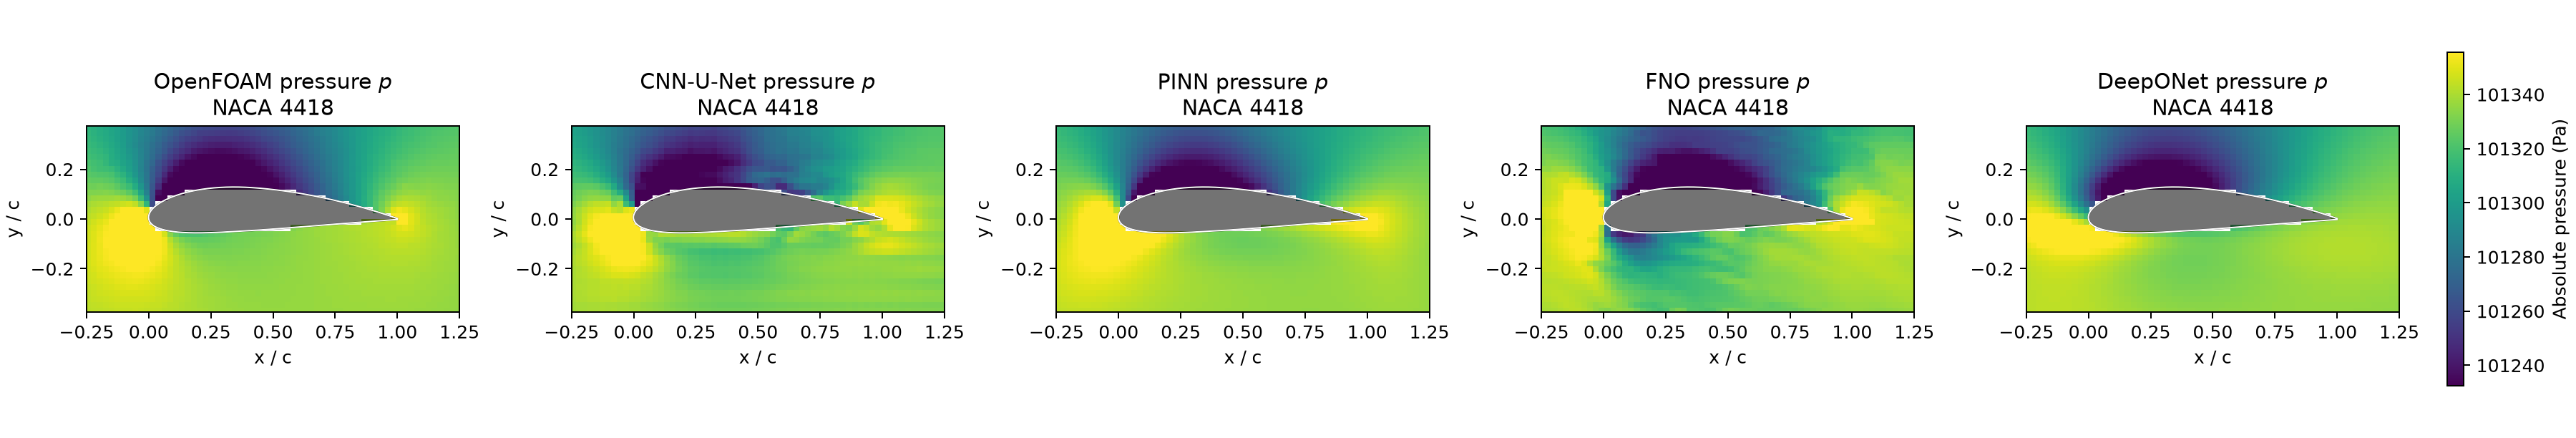
\includegraphics[width=0.98\textwidth]{figures/heldout_pressure.png}
\caption{Absolute-pressure prediction for NACA 4418. The view spans $x/c\in[-0.25,1.25]$ and
$y/c\in[-0.375,0.375]$.}
\label{fig:pressure}
\end{figure*}

\subsection{Cavitation-inception screening}
The pressure-threshold labels are highly imbalanced, so we report F1 rather
than accuracy. DeepONet obtains $0.900\pm0.008$, the PINN
$0.859\pm0.015$, CNN-U-Net $0.758\pm0.198$, and FNO $0.724\pm0.065$. This is a
secondary low-$C_p$ diagnostic, not a prediction of cavity dynamics
\citep{brennen1995cavitation}.

\subsection{Shape optimization against direct CFD}
Figure~\ref{fig:optimization} reports the complete $L/D$ comparison: the
OpenFOAM value of the starting foil, the surrogate estimate at its selected
design, and the result of remeshing that design and solving it once in
OpenFOAM. This one-solve endpoint check is distinct from the direct baseline,
which places OpenFOAM inside the matched optimizer.

Across three selected endpoints per architecture, medium-grid OpenFOAM gives
$L/D=24.44\pm1.35$ for CNN-U-Net, $36.85\pm5.09$ for the PINN,
$22.10\pm3.46$ for FNO, and $37.47\pm5.95$ for DeepONet. The matched
direct-CFD search reaches 29.89. These values are not mesh-independent: on the
seed-7 winners, medium-to-fine $L/D$ shifts are 16--22\%.

\begin{figure}[t]
\centering
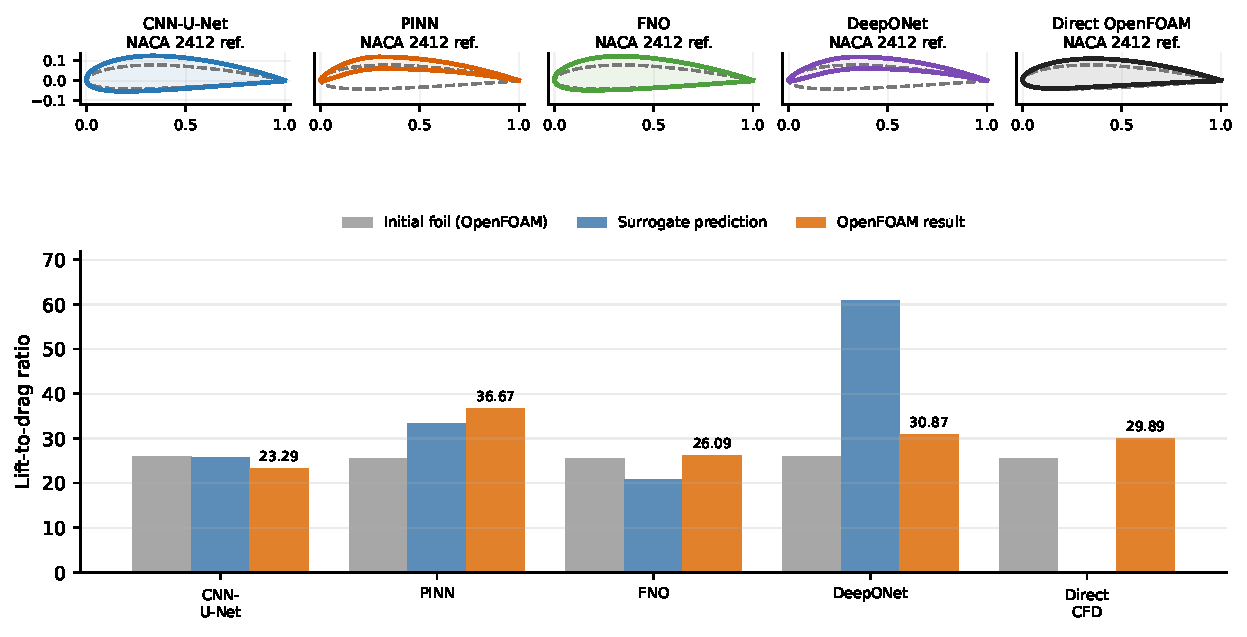
\includegraphics[width=0.82\textwidth]{figures/aso_results.pdf}
\caption{Top: selected shapes against the same dashed NACA 2412 geometric
reference. The reference is for visual comparison, not necessarily the
optimizer initializer. Bottom: initial-foil OpenFOAM values, surrogate
predictions, fresh OpenFOAM endpoint checks, and direct CFD.}
\label{fig:optimization}
\end{figure}

\section{Discussion}
DeepONet is the best final-test predictor, while its optimized endpoints and
those of the PINN both vary across seeds. CNN-U-Net is
unstable in both force prediction and optimization; FNO is more repeatable but
selects lower-performing designs. Accuracy, candidate ranking, and seed
robustness are therefore distinct.

All 12 three-level grid-study runs converge iteratively by 1,000 iterations,
with maximum final initial residuals below $10^{-5}$ and force spans below
$3\times10^{-6}$ over the final 50 iterations. Lift changes by at
most about 4\% from medium to fine, but drag changes by 16--26\%. Thus, a fresh
OpenFOAM endpoint is a standard and useful verification step, yet it is not by
itself a grid-independent validation. This is precisely the simulator
imperfection exposed by carrying the benchmark through the design loop.

The continuous optimizer also queries descriptors between and near the bounds
of twelve discrete families. Endpoint CFD checks the selected shape, not the
entire learned surface. All winners remain far from vapor pressure, so
cavitation is a secondary diagnostic rather than an active constraint. The
rankings are therefore evidence for this controlled benchmark, not for general
hydrofoil design: the remaining scope is steady 2D RANS, one compact
configuration per architecture, three seeds, and the NACA four-digit space.

\section{Conclusion}
While standard benchmarks rank neural flow surrogates by field and force errors---where DeepONet excels and the compact PINN dominates in speed---our end-to-end evaluation reveals a critical blind spot. Pushing these models through a multi-start optimization loop demonstrates that isolated test accuracy does not reliably predict downstream design decisions or seed robustness. To truly bridge machine learning and scientific engineering, surrogates must be evaluated on their operational consequences and the numerical uncertainty of the verifying simulator. Future work will advance this paradigm through three-dimensional flows and active cavitation-constrained optimization.

\bibliographystyle{plainnat}
\bibliography{references}

\appendix
\section{Code and data availability}
Source code and reproduction instructions are available at
\url{https://github.com/aaravvd/hydrofoil-neural-surrogates}. The CFD dataset
and trained checkpoints are archived at
\url{https://doi.org/10.5281/zenodo.21845241}. Code is released under the MIT
License; generated data and checkpoints use CC BY 4.0.

\section{PINN objective}
\label{app:physics}
The network predicts normalized outputs, but the residuals are evaluated after
velocity and pressure are returned to physical units. For output channel $q$,
\begin{equation}
q=\sigma_q\widehat q+\mu_q,
\qquad
\frac{\partial q}{\partial x_i}
=\frac{\sigma_q}{\sigma_{x_i}}
\frac{\partial\widehat q}{\partial\widehat x_i},
\end{equation}
where the means and standard deviations are computed from the training set.
Comma subscripts denote partial spatial derivatives. Let
$\nu_e=\nu+\max(\nu_t,0)$. The modeled kinematic stresses are
\begin{align}
\tau_{xx}&=2\nu_e U_{x,x},\qquad
\tau_{xy}=\nu_e(U_{x,y}+U_{y,x}),\\
\tau_{yy}&=2\nu_e U_{y,y}.
\end{align}
The sampled-point continuity and momentum residuals are
\begin{align}
r_c&=U_{x,x}+U_{y,y},\\
r_x&=U_xU_{x,x}+U_yU_{x,y}+p_{,x}/\rho-\tau_{xx,x}-\tau_{xy,y},\\
r_y&=U_xU_{y,x}+U_yU_{y,y}+p_{,y}/\rho-\tau_{xy,x}-\tau_{yy,y}.
\end{align}
For chord $c$ and casewise freestream speed $U_\infty$, the combined objective is
\begin{equation}
\mathcal{L}=\mathcal{L}_{\mathrm{sup}}+10^{-4}
\left[\operatorname{MSE}\!\left(\frac{c r_c}{U_\infty}\right)
+\operatorname{MSE}\!\left(\frac{c r_x}{U_\infty^2}\right)
+\operatorname{MSE}\!\left(\frac{c r_y}{U_\infty^2}\right)\right].
\end{equation}

\clearpage
\section{Complete optimization traces}
\begin{figure}[h]
\centering
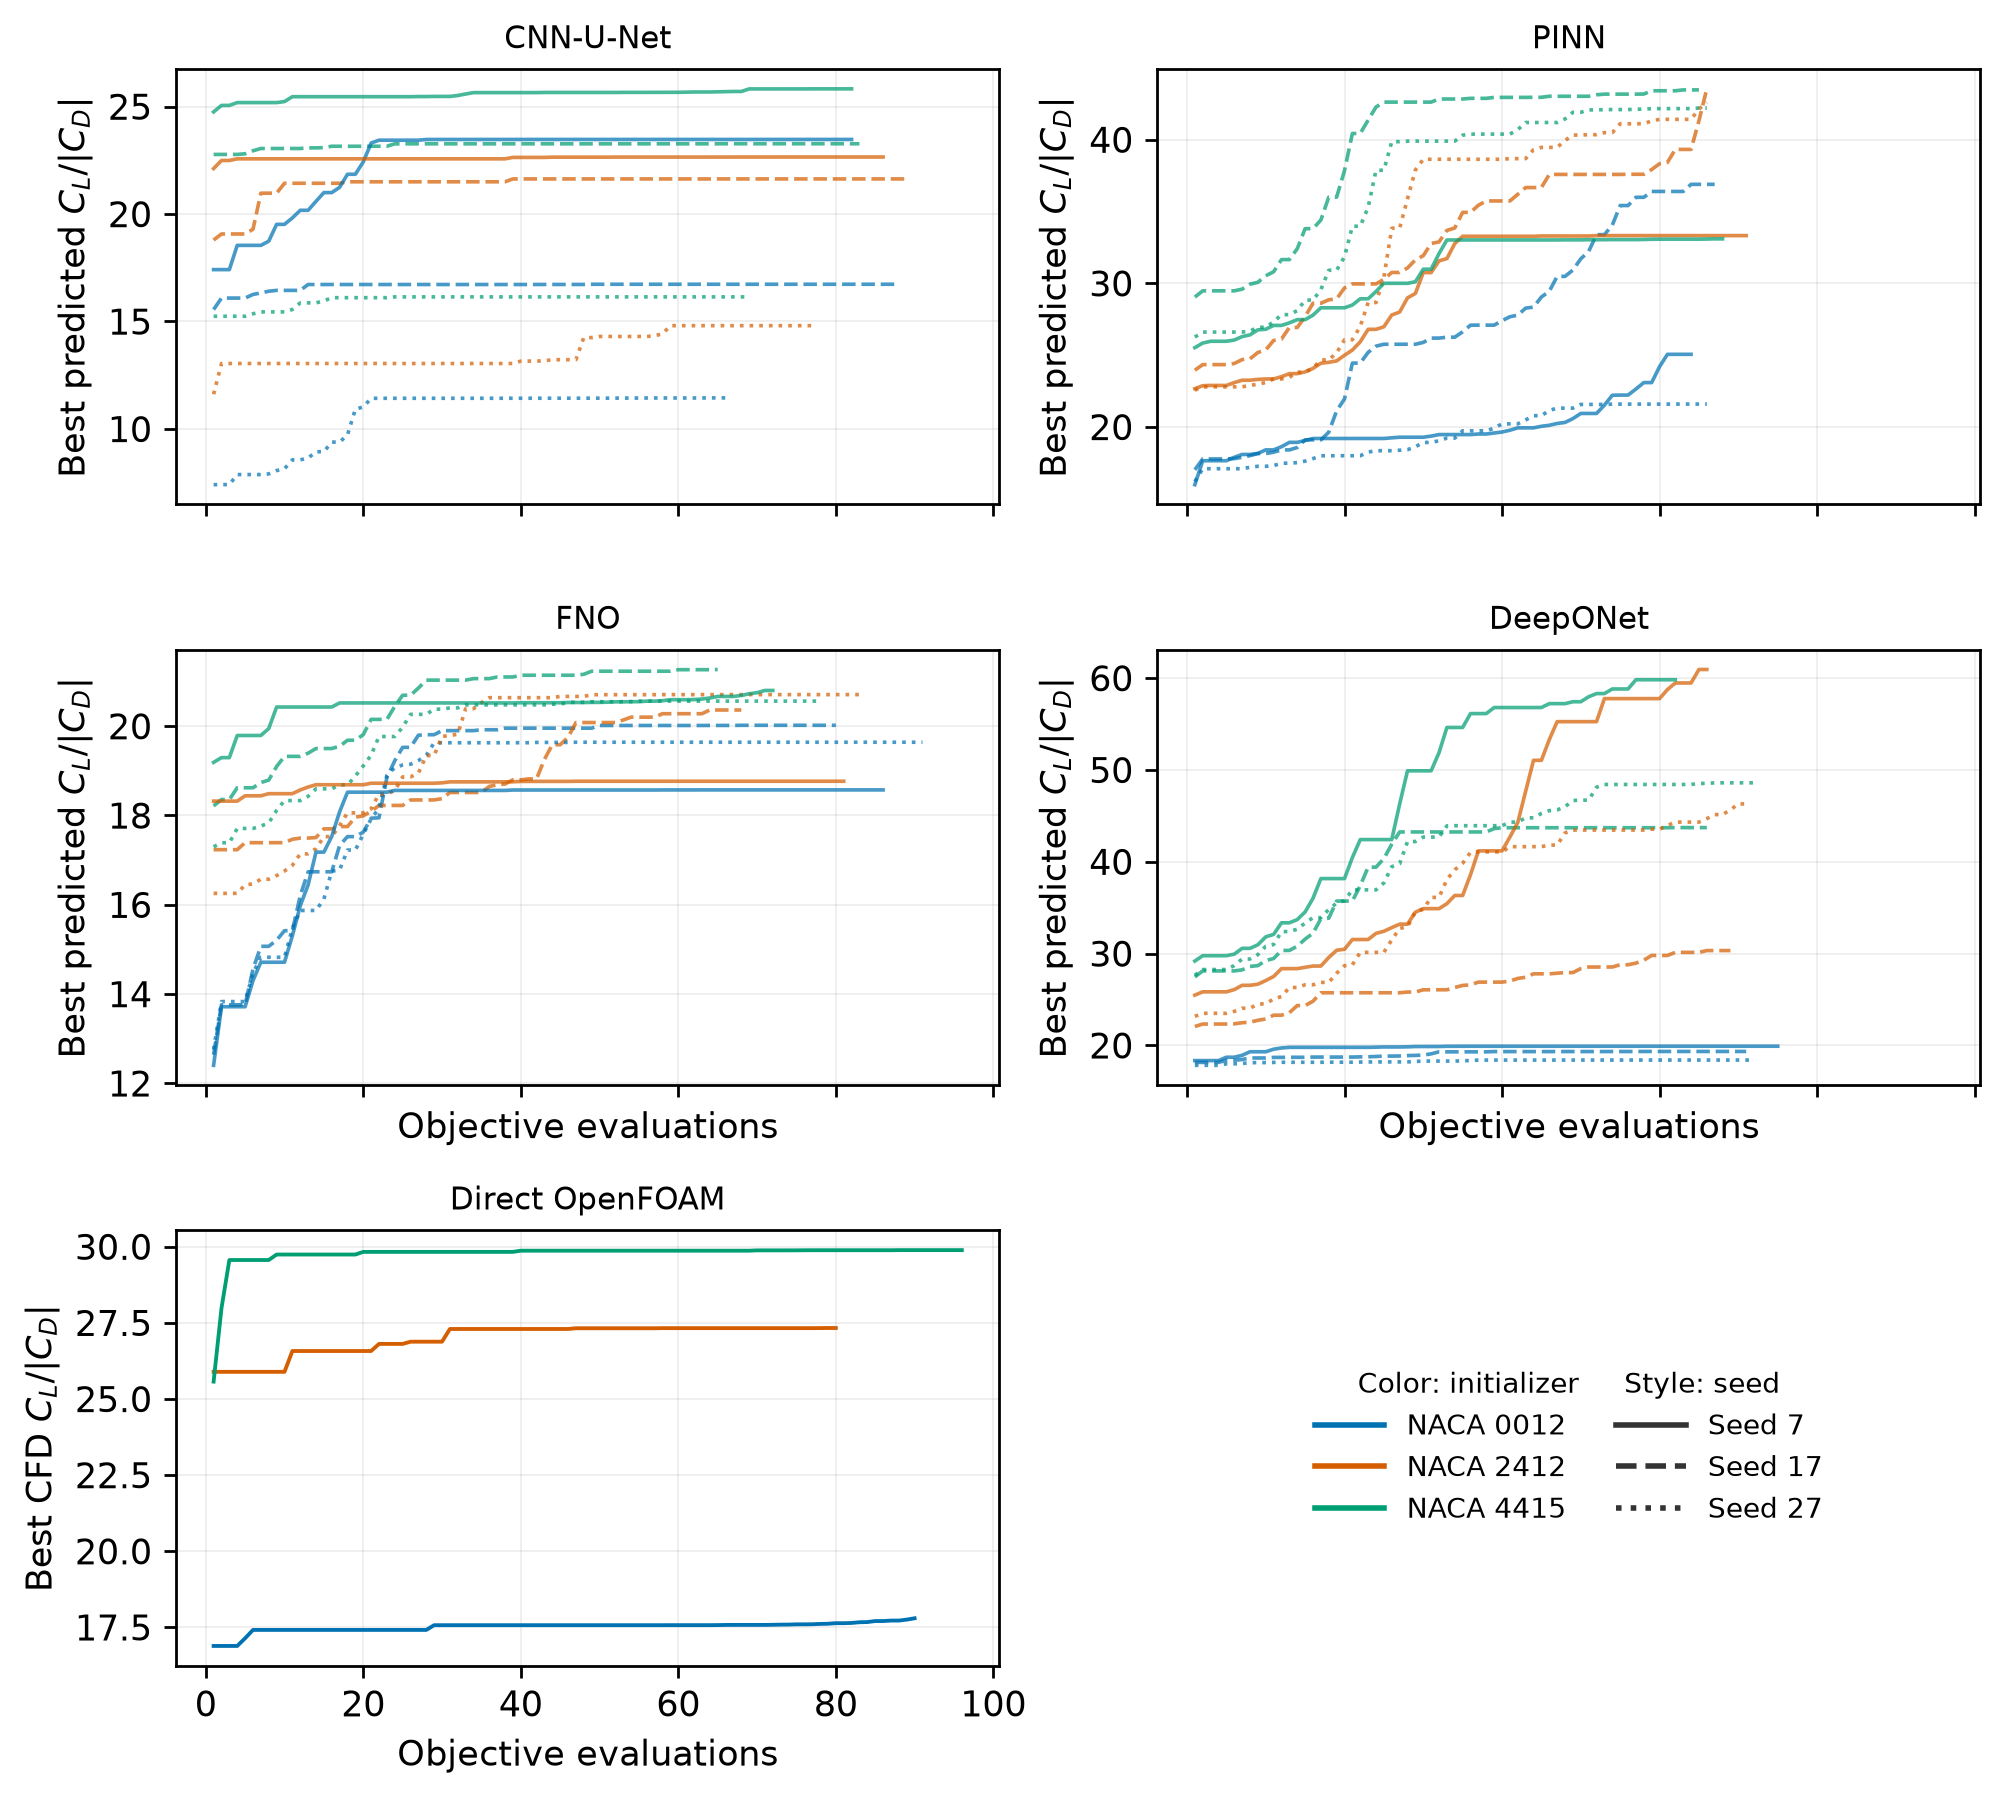
\includegraphics[width=0.98\textwidth]{figures/optimization_traces.png}
\caption{All three optimization starts and three training seeds per surrogate,
with the three direct-CFD starts. Color identifies the NACA 0012, 2412, or 4415
initializer; the three same-color surrogate curves correspond to seeds 7, 17,
and 27. Lines show the best-so-far objective, and every raw evaluation is
available in the public repository.}
\label{fig:traces}
\end{figure}

\clearpage
\section*{NeurIPS Paper Checklist}

\begin{enumerate}

\item {\bf Claims}
    \item[] Question: Do the main claims made in the abstract and introduction accurately reflect the paper's contributions and scope?
    \item[] Answer: \answerYes{}
    \item[] Justification: The abstract, introduction, and limitations distinguish CFD agreement, physical validation, and pressure-based inception screening.
    \item[] Guidelines:
    \begin{itemize}
        \item The answer \answerNA{} means that the abstract and introduction do not include the claims made in the paper.
        \item The abstract and/or introduction should clearly state the claims made, including the contributions made in the paper and important assumptions and limitations. A \answerNo{} or \answerNA{} answer to this question will not be perceived well by the reviewers. 
        \item The claims made should match theoretical and experimental results, and reflect how much the results can be expected to generalize to other settings. 
        \item It is fine to include aspirational goals as motivation as long as it is clear that these goals are not attained by the paper. 
    \end{itemize}

\item {\bf Limitations}
    \item[] Question: Does the paper discuss the limitations of the work performed by the authors?
    \item[] Answer: \answerYes{}
    \item[] Justification: Section 5 discusses simulator fidelity, geometry scope, direct force supervision, continuous-shape extrapolation, and the boundary of the cavitation diagnostic.
    \item[] Guidelines:
    \begin{itemize}
        \item The answer \answerNA{} means that the paper has no limitation while the answer \answerNo{} means that the paper has limitations, but those are not discussed in the paper. 
        \item The authors are encouraged to create a separate ``Limitations'' section in their paper.
        \item The paper should point out any strong assumptions and how robust the results are to violations of these assumptions (e.g., independence assumptions, noiseless settings, model well-specification, asymptotic approximations only holding locally). The authors should reflect on how these assumptions might be violated in practice and what the implications would be.
        \item The authors should reflect on the scope of the claims made, e.g., if the approach was only tested on a few datasets or with a few runs. In general, empirical results often depend on implicit assumptions, which should be articulated.
        \item The authors should reflect on the factors that influence the performance of the approach. For example, a facial recognition algorithm may perform poorly when image resolution is low or images are taken in low lighting. Or a speech-to-text system might not be used reliably to provide closed captions for online lectures because it fails to handle technical jargon.
        \item The authors should discuss the computational efficiency of the proposed algorithms and how they scale with dataset size.
        \item If applicable, the authors should discuss possible limitations of their approach to address problems of privacy and fairness.
        \item While the authors might fear that complete honesty about limitations might be used by reviewers as grounds for rejection, a worse outcome might be that reviewers discover limitations that aren't acknowledged in the paper. The authors should use their best judgment and recognize that individual actions in favor of transparency play an important role in developing norms that preserve the integrity of the community. Reviewers will be specifically instructed to not penalize honesty concerning limitations.
    \end{itemize}

\item {\bf Theory assumptions and proofs}
    \item[] Question: For each theoretical result, does the paper provide the full set of assumptions and a complete (and correct) proof?
    \item[] Answer: \answerNA{}
    \item[] Justification: The paper presents an empirical benchmark and no theoretical results or proofs.
    \item[] Guidelines:
    \begin{itemize}
        \item The answer \answerNA{} means that the paper does not include theoretical results. 
        \item All the theorems, formulas, and proofs in the paper should be numbered and cross-referenced.
        \item All assumptions should be clearly stated or referenced in the statement of any theorems.
        \item The proofs can either appear in the main paper or the supplemental material, but if they appear in the supplemental material, the authors are encouraged to provide a short proof sketch to provide intuition. 
        \item Inversely, any informal proof provided in the core of the paper should be complemented by formal proofs provided in appendix or supplemental material.
        \item Theorems and Lemmas that the proof relies upon should be properly referenced. 
    \end{itemize}

    \item {\bf Experimental result reproducibility}
    \item[] Question: Does the paper fully disclose all the information needed to reproduce the main experimental results of the paper to the extent that it affects the main claims and/or conclusions of the paper (regardless of whether the code and data are provided or not)?
    \item[] Answer: \answerYes{}
    \item[] Justification: Sections 2--3 specify the case matrix, split, CFD setup, model families, losses, hyperparameters, and optimization protocol.
    \item[] Guidelines:
    \begin{itemize}
        \item The answer \answerNA{} means that the paper does not include experiments.
        \item If the paper includes experiments, a \answerNo{} answer to this question will not be perceived well by the reviewers: Making the paper reproducible is important, regardless of whether the code and data are provided or not.
        \item If the contribution is a dataset and\slash or model, the authors should describe the steps taken to make their results reproducible or verifiable. 
        \item Depending on the contribution, reproducibility can be accomplished in various ways. For example, if the contribution is a novel architecture, describing the architecture fully might suffice, or if the contribution is a specific model and empirical evaluation, it may be necessary to either make it possible for others to replicate the model with the same dataset, or provide access to the model. In general. releasing code and data is often one good way to accomplish this, but reproducibility can also be provided via detailed instructions for how to replicate the results, access to a hosted model (e.g., in the case of a large language model), releasing of a model checkpoint, or other means that are appropriate to the research performed.
        \item While NeurIPS does not require releasing code, the conference does require all submissions to provide some reasonable avenue for reproducibility, which may depend on the nature of the contribution. For example
        \begin{enumerate}
            \item If the contribution is primarily a new algorithm, the paper should make it clear how to reproduce that algorithm.
            \item If the contribution is primarily a new model architecture, the paper should describe the architecture clearly and fully.
            \item If the contribution is a new model (e.g., a large language model), then there should either be a way to access this model for reproducing the results or a way to reproduce the model (e.g., with an open-source dataset or instructions for how to construct the dataset).
            \item We recognize that reproducibility may be tricky in some cases, in which case authors are welcome to describe the particular way they provide for reproducibility. In the case of closed-source models, it may be that access to the model is limited in some way (e.g., to registered users), but it should be possible for other researchers to have some path to reproducing or verifying the results.
        \end{enumerate}
    \end{itemize}


\item {\bf Open access to data and code}
    \item[] Question: Does the paper provide open access to the data and code, with sufficient instructions to faithfully reproduce the main experimental results, as described in supplemental material?
    \item[] Answer: \answerYes{}
    \item[] Justification: Appendix A links the public repository and release, which provide three checkpoints per architecture, final-test grids, compact results, licenses, and exact reproduction instructions: \url{https://github.com/aaravvd/hydrofoil-neural-surrogates/releases/tag/sim2science2026-camera-ready}.
    \item[] Guidelines:
    \begin{itemize}
        \item The answer \answerNA{} means that paper does not include experiments requiring code.
        \item Please see the NeurIPS code and data submission guidelines (\url{https://neurips.cc/public/guides/CodeSubmissionPolicy}) for more details.
        \item While we encourage the release of code and data, we understand that this might not be possible, so \answerNo{} is an acceptable answer. Papers cannot be rejected simply for not including code, unless this is central to the contribution (e.g., for a new open-source benchmark).
        \item The instructions should contain the exact command and environment needed to run to reproduce the results. See the NeurIPS code and data submission guidelines (\url{https://neurips.cc/public/guides/CodeSubmissionPolicy}) for more details.
        \item The authors should provide instructions on data access and preparation, including how to access the raw data, preprocessed data, intermediate data, and generated data, etc.
        \item The authors should provide scripts to reproduce all experimental results for the new proposed method and baselines. If only a subset of experiments are reproducible, they should state which ones are omitted from the script and why.
        \item At submission time, to preserve anonymity, the authors should release anonymized versions (if applicable).
        \item Providing as much information as possible in supplemental material (appended to the paper) is recommended, but including URLs to data and code is permitted.
    \end{itemize}


\item {\bf Experimental setting/details}
    \item[] Question: Does the paper specify all the training and test details (e.g., data splits, hyperparameters, how they were chosen, type of optimizer) necessary to understand the results?
    \item[] Answer: \answerYes{}
    \item[] Justification: Sections 2--3 give the fixed train/validation/test families, three seeds, optimizer, learning rate, model sizes, stopping rule, and design bounds.
    \item[] Guidelines:
    \begin{itemize}
        \item The answer \answerNA{} means that the paper does not include experiments.
        \item The experimental setting should be presented in the core of the paper to a level of detail that is necessary to appreciate the results and make sense of them.
        \item The full details can be provided either with the code, in appendix, or as supplemental material.
    \end{itemize}

\item {\bf Experiment statistical significance}
    \item[] Question: Does the paper report error bars suitably and correctly defined or other appropriate information about the statistical significance of the experiments?
    \item[] Answer: \answerYes{}
    \item[] Justification: Every architecture is trained with seeds 7, 17, and 27 on the same split; tables report the mean and one sample standard deviation over those independent training runs.
    \item[] Guidelines:
    \begin{itemize}
        \item The answer \answerNA{} means that the paper does not include experiments.
        \item The authors should answer \answerYes{} if the results are accompanied by error bars, confidence intervals, or statistical significance tests, at least for the experiments that support the main claims of the paper.
        \item The factors of variability that the error bars are capturing should be clearly stated (for example, train/test split, initialization, random drawing of some parameter, or overall run with given experimental conditions).
        \item The method for calculating the error bars should be explained (closed form formula, call to a library function, bootstrap, etc.)
        \item The assumptions made should be given (e.g., Normally distributed errors).
        \item It should be clear whether the error bar is the standard deviation or the standard error of the mean.
        \item It is OK to report 1-sigma error bars, but one should state it. The authors should preferably report a 2-sigma error bar than state that they have a 96\% CI, if the hypothesis of Normality of errors is not verified.
        \item For asymmetric distributions, the authors should be careful not to show in tables or figures symmetric error bars that would yield results that are out of range (e.g., negative error rates).
        \item If error bars are reported in tables or plots, the authors should explain in the text how they were calculated and reference the corresponding figures or tables in the text.
    \end{itemize}

\item {\bf Experiments compute resources}
    \item[] Question: For each experiment, does the paper provide sufficient information on the computer resources (type of compute workers, memory, time of execution) needed to reproduce the experiments?
    \item[] Answer: \answerYes{}
    \item[] Justification: Section 4 reports CPU hardware, memory, software versions, training time, solver time, inference time, and amortized break-even counts.
    \item[] Guidelines:
    \begin{itemize}
        \item The answer \answerNA{} means that the paper does not include experiments.
        \item The paper should indicate the type of compute workers CPU or GPU, internal cluster, or cloud provider, including relevant memory and storage.
        \item The paper should provide the amount of compute required for each of the individual experimental runs as well as estimate the total compute. 
        \item The paper should disclose whether the full research project required more compute than the experiments reported in the paper (e.g., preliminary or failed experiments that didn't make it into the paper). 
    \end{itemize}
    
\item {\bf Code of ethics}
    \item[] Question: Does the research conducted in the paper conform, in every respect, with the NeurIPS Code of Ethics \url{https://neurips.cc/public/EthicsGuidelines}?
    \item[] Answer: \answerYes{}
    \item[] Justification: The research uses generated CFD data, involves no people or sensitive data, and preserves limitations and exclusions.
    \item[] Guidelines:
    \begin{itemize}
        \item The answer \answerNA{} means that the authors have not reviewed the NeurIPS Code of Ethics.
        \item If the authors answer \answerNo, they should explain the special circumstances that require a deviation from the Code of Ethics.
        \item The authors should make sure to preserve anonymity (e.g., if there is a special consideration due to laws or regulations in their jurisdiction).
    \end{itemize}


\item {\bf Broader impacts}
    \item[] Question: Does the paper discuss both potential positive societal impacts and negative societal impacts of the work performed?
    \item[] Answer: \answerYes{}
    \item[] Justification: Section 5 discusses computational benefits and the risk that surrogate speed can scale simulator bias or invalid cavitation claims.
    \item[] Guidelines:
    \begin{itemize}
        \item The answer \answerNA{} means that there is no societal impact of the work performed.
        \item If the authors answer \answerNA{} or \answerNo, they should explain why their work has no societal impact or why the paper does not address societal impact.
        \item Examples of negative societal impacts include potential malicious or unintended uses (e.g., disinformation, generating fake profiles, surveillance), fairness considerations (e.g., deployment of technologies that could make decisions that unfairly impact specific groups), privacy considerations, and security considerations.
        \item The conference expects that many papers will be foundational research and not tied to particular applications, let alone deployments. However, if there is a direct path to any negative applications, the authors should point it out. For example, it is legitimate to point out that an improvement in the quality of generative models could be used to generate Deepfakes for disinformation. On the other hand, it is not needed to point out that a generic algorithm for optimizing neural networks could enable people to train models that generate Deepfakes faster.
        \item The authors should consider possible harms that could arise when the technology is being used as intended and functioning correctly, harms that could arise when the technology is being used as intended but gives incorrect results, and harms following from (intentional or unintentional) misuse of the technology.
        \item If there are negative societal impacts, the authors could also discuss possible mitigation strategies (e.g., gated release of models, providing defenses in addition to attacks, mechanisms for monitoring misuse, mechanisms to monitor how a system learns from feedback over time, improving the efficiency and accessibility of ML).
    \end{itemize}
    
\item {\bf Safeguards}
    \item[] Question: Does the paper describe safeguards that have been put in place for responsible release of data or models that have a high risk for misuse (e.g., pre-trained language models, image generators, or scraped datasets)?
    \item[] Answer: \answerNA{}
    \item[] Justification: The generated hydrofoil models and CFD fields do not present a high-risk dual-use release.
    \item[] Guidelines:
    \begin{itemize}
        \item The answer \answerNA{} means that the paper poses no such risks.
        \item Released models that have a high risk for misuse or dual-use should be released with necessary safeguards to allow for controlled use of the model, for example by requiring that users adhere to usage guidelines or restrictions to access the model or implementing safety filters. 
        \item Datasets that have been scraped from the Internet could pose safety risks. The authors should describe how they avoided releasing unsafe images.
        \item We recognize that providing effective safeguards is challenging, and many papers do not require this, but we encourage authors to take this into account and make a best faith effort.
    \end{itemize}

\item {\bf Licenses for existing assets}
    \item[] Question: Are the creators or original owners of assets (e.g., code, data, models), used in the paper, properly credited and are the license and terms of use explicitly mentioned and properly respected?
    \item[] Answer: \answerYes{}
    \item[] Justification: OpenFOAM and the prior architectures are cited; dependency versions are pinned, source code is MIT licensed, and the generated dataset and checkpoints are CC BY 4.0 licensed in the artifact.
    \item[] Guidelines:
    \begin{itemize}
        \item The answer \answerNA{} means that the paper does not use existing assets.
        \item The authors should cite the original paper that produced the code package or dataset.
        \item The authors should state which version of the asset is used and, if possible, include a URL.
        \item The name of the license (e.g., CC-BY 4.0) should be included for each asset.
        \item For scraped data from a particular source (e.g., website), the copyright and terms of service of that source should be provided.
        \item If assets are released, the license, copyright information, and terms of use in the package should be provided. For popular datasets, \url{paperswithcode.com/datasets} has curated licenses for some datasets. Their licensing guide can help determine the license of a dataset.
        \item For existing datasets that are re-packaged, both the original license and the license of the derived asset (if it has changed) should be provided.
        \item If this information is not available online, the authors are encouraged to reach out to the asset's creators.
    \end{itemize}

\item {\bf New assets}
    \item[] Question: Are new assets introduced in the paper well documented and is the documentation provided alongside the assets?
    \item[] Answer: \answerYes{}
    \item[] Justification: The public repository and data archive document generation, fixed family partition, training, evaluation, optimization, CFD checks, expected outputs, claim boundaries, and separate code/data licenses.
    \item[] Guidelines:
    \begin{itemize}
        \item The answer \answerNA{} means that the paper does not release new assets.
        \item Researchers should communicate the details of the dataset\slash code\slash model as part of their submissions via structured templates. This includes details about training, license, limitations, etc. 
        \item The paper should discuss whether and how consent was obtained from people whose asset is used.
        \item At submission time, remember to anonymize your assets (if applicable). You can either create an anonymized URL or include an anonymized zip file.
    \end{itemize}

\item {\bf Crowdsourcing and research with human subjects}
    \item[] Question: For crowdsourcing experiments and research with human subjects, does the paper include the full text of instructions given to participants and screenshots, if applicable, as well as details about compensation (if any)? 
    \item[] Answer: \answerNA{}
    \item[] Justification: The work contains no crowdsourcing or human-subject research.
    \item[] Guidelines:
    \begin{itemize}
        \item The answer \answerNA{} means that the paper does not involve crowdsourcing nor research with human subjects.
        \item Including this information in the supplemental material is fine, but if the main contribution of the paper involves human subjects, then as much detail as possible should be included in the main paper. 
        \item According to the NeurIPS Code of Ethics, workers involved in data collection, curation, or other labor should be paid at least the minimum wage in the country of the data collector. 
    \end{itemize}

\item {\bf Institutional review board (IRB) approvals or equivalent for research with human subjects}
    \item[] Question: Does the paper describe potential risks incurred by study participants, whether such risks were disclosed to the subjects, and whether Institutional Review Board (IRB) approvals (or an equivalent approval/review based on the requirements of your country or institution) were obtained?
    \item[] Answer: \answerNA{}
    \item[] Justification: The work contains no human-subject research requiring IRB review.
    \item[] Guidelines:
    \begin{itemize}
        \item The answer \answerNA{} means that the paper does not involve crowdsourcing nor research with human subjects.
        \item Depending on the country in which research is conducted, IRB approval (or equivalent) may be required for any human subjects research. If you obtained IRB approval, you should clearly state this in the paper. 
        \item We recognize that the procedures for this may vary significantly between institutions and locations, and we expect authors to adhere to the NeurIPS Code of Ethics and the guidelines for their institution. 
        \item For initial submissions, do not include any information that would break anonymity (if applicable), such as the institution conducting the review.
    \end{itemize}

\item {\bf Declaration of LLM usage}
    \item[] Question: Does the paper describe the usage of LLMs if it is an important, original, or non-standard component of the core methods in this research? Note that if the LLM is used only for writing, editing, or formatting purposes and does \emph{not} impact the core methodology, scientific rigor, or originality of the research, declaration is not required.
    %this research? 
    \item[] Answer: \answerNA{}
    \item[] Justification: LLMs are not part of the scientific method, model architectures, data generation, or evaluation reported in the paper.
    \item[] Guidelines:
    \begin{itemize}
        \item The answer \answerNA{} means that the core method development in this research does not involve LLMs as any important, original, or non-standard components.
        \item Please refer to our LLM policy in the NeurIPS handbook for what should or should not be described.
    \end{itemize}

\end{enumerate}


\end{document}
